% zip letter-value-plot.zip *.tex *.bib code-data images
\documentclass[12pt,oneside]{article}
\usepackage{fullpage}

\usepackage{hyperref}
\usepackage{booktabs}
\usepackage[format=plain,font=small]{caption}
\usepackage[small]{titlesec}
\usepackage[round,sectionbib]{natbib}
\usepackage{setspace}
\renewcommand\rmdefault{bch}
\linespread{2} 
\usepackage{amssymb}
\usepackage{amsthm}
\newcommand{\Reals}{{\rm I\kern-.1667em{}R}}
\usepackage[pdftex]{graphicx}
\DeclareGraphicsExtensions{.png,.pdf}
\graphicspath{{images/}}

\title{Letter-value plots: Boxplots for large datasets}
\author{\begin{tabular}[t]{c c c }
  Heike Hofmann         & Karen Kafadar         & Hadley Wickham \\
  Dept of Statistics    & Dept of Statistics    & Dept of Statistics \\
  Iowa State University & Indiana University    & Rice University \\
  Ames, IA 50011        & Bloomington, IN 47408 & Houston, TX 77001
\end{tabular}}

\pdfminorversion=4
\begin{document}
\maketitle

\begin{abstract}

  Conventional boxplots \citep{eda} are useful displays for conveying rough
  information about the central 50\% and the extent of data. For small-sized
  data sets ($n < 200$), detailed estimates of tail behavior beyond the
  quartiles may not be trustworthy, so the information provided by boxplots is
  appropriately somewhat vague beyond the quartiles, and the expected number
  of ``outliers'' of size $n$ is often less than 10 \citep{dchbox}. Larger
  data sets ($n \approx 10,000$--$100,000$) afford more precise estimates of
  quantiles beyond the quartiles, but conventional boxplots do not show this
  information about the tails, and, in addition, show large numbers of
  extreme, but not unexpected, observations.

  The letter-value plot addresses both of these shortcomings: (1) it conveys more
  detailed information in the tails using letter values, but only to the
  depths where the letter values are reliable estimates of their corresponding
  quantiles and (2) outliers are labeled as those observations beyond the
  most extreme letter value. All features shown on the letter-value plot are
  actual observations, thus remaining faithful to the principles that governed
  Tukey's original boxplot. We illustrate letter-value plots on real data
  (univariate and bivariate) that demonstrate their usefulness, particularly
  for large data sets. All graphics are created using R \citep{R2011}.
Code and data are available in the supplementary materials.

  \textbf{Key words}: boxplots, quantiles, letter value display, 
  fourth, order statistics, tail area, location depth.
  
\end{abstract}

\tableofcontents
\section{Introduction}

Boxplots \citep{tukey:1970,tukey72} are one of the few statistical graphics invented in the 20th century
that have gained widespread adoption. Despite their widespread use, they are
not altogether satisfactory, particularly for large data sets. Specifically,
two problems arise with boxplots when applied to large data sets: (1) the
number of outlier (observations beyond the whiskers) grows linearly with
the sample size and (2) estimates of tail behavior are not displayed, despite
the fact that larger sample sizes allow more reliable estimates further out
into the tails. 




%Figure~\ref{fig:internet-bp} illustrates both problems with a
%boxplot of 135,605 internet (log-transformed) session durations, stratified
%into 32 groups based on the logarithm of the number of bytes transferred
%during the session. See \citet{kw06} for further details about the data and
%transformations. The sample sizes in the 32 boxes range from 1341 (box \#32)
%to 7865 (Box \#13), with a median sample size of 4238. 
Figure \ref{fig:taxi-bp} illustrates both of these problems.  (Square root) taxi times  for 478,755 US national flights in January 2012 are shown in boxplots by airline carriers.  Carriers are ordered according to number of flights served left to right. The largest three carriers, WN (Southwest), EV (ExpressJet)  and DL (Delta) show striking differences in the median taxi times -- Southwest is with a median taxi time of 3.74$^2$ = 14 minutes well below the overall median of 20 minutes, whereas Delta has a median taxi time of 25 minutes and is significantly above the overall median.

The sample sizes in the fifteen groups vary between 4,062 flights by VX (Virgin America) and 89,920 flights by Southwest, WN. 
With so many
observations in each group, the number of labeled outliers is huge, with
far too many to investigate individually, making it difficult to distinguish
between extreme values and true outliers.

%\begin{figure}[hbtp]
%  \centering
%  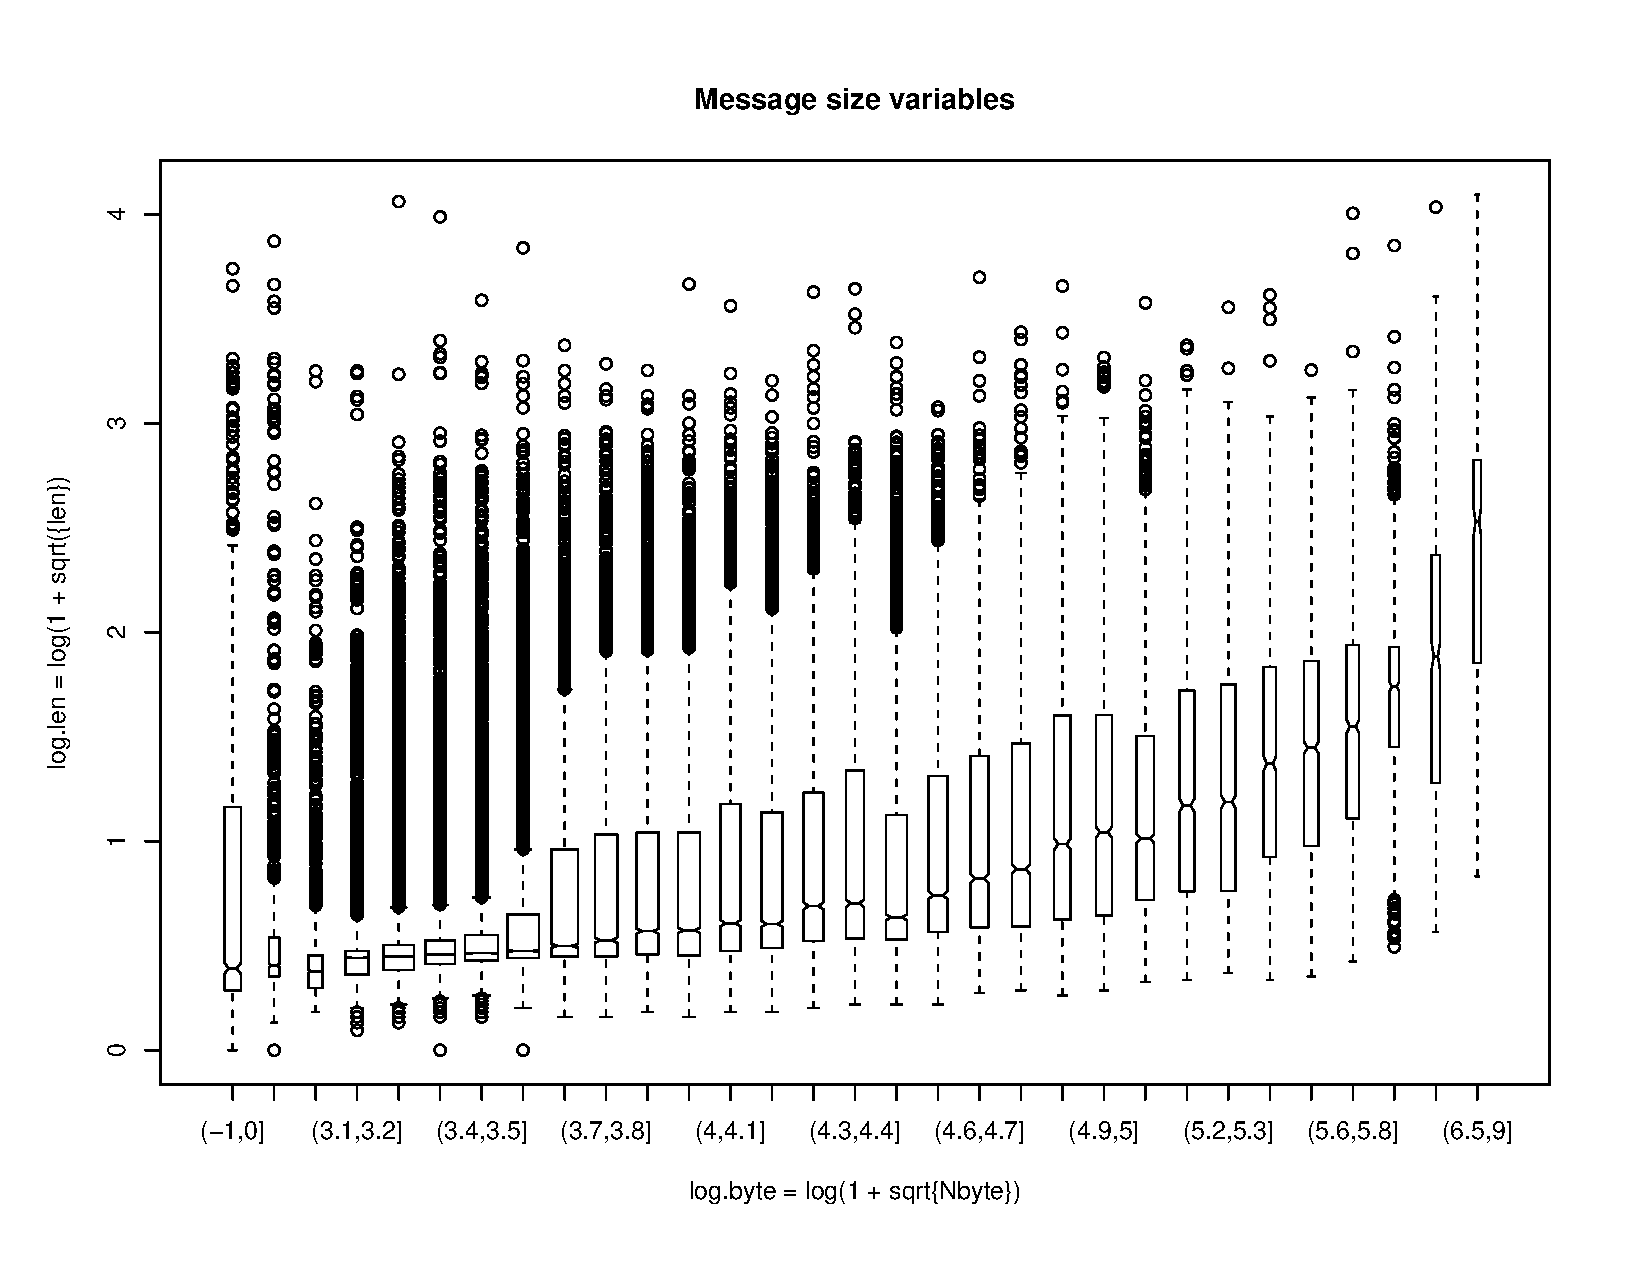
\includegraphics[width=\linewidth]{box2}
%
%  \caption{Notched boxplots \citep{variations.boxplots} of (log-transformed)
%  duration for 135,605 internet sessions, grouped by ranges of
%  (log-transformed) byte lengths for the sessions.}
%
%  \label{fig:internet-bp} 
%\end{figure}

\begin{figure}[hbtp]
  \centering
  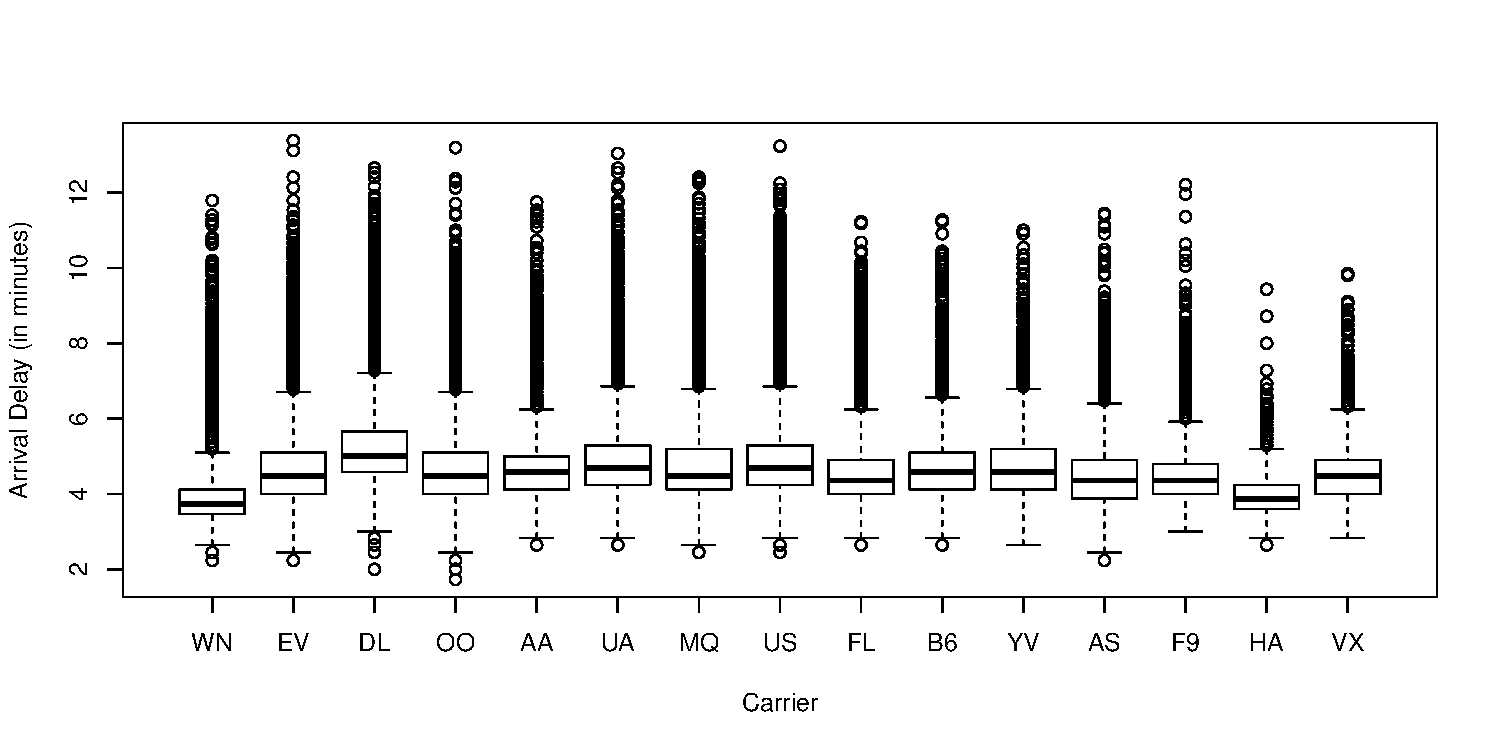
\includegraphics[width=\linewidth]{taxi-bp}

  \caption{Notched boxplots \citep{variations.boxplots} of (sqrt-transformed)
  taxi in and out times grouped by airline carrier for flights in January 2012. Airline carriers are ordered left to right in decreasing  number of flights served. }

  \label{fig:taxi-bp} 
\end{figure}


%Boxplots \citep{tukey:1970,tukey72} give a compact graphical summary of the distribution of a variable, based around a set of order statistics called letter values. In \textit{Exploratory Data Analysis}, \citet{eda} recommended the $([n/2] + 1)/2$-th and $(n + 1 - ([n/2] + 1)/2)$-th order statistics as estimates of the quartiles, the ``lower fourth'' and ``upper fourth'' in \citet{ureda} with \textit{depth} $([n/2] + 1)/2$ because they lie that many observations in from the extremes.  
The definition of boxplots is based around a set of order statistics called letter values -- in particular, the median, $M$, and the fourths, $F$.  
\citet{eda} recommended in \textit{Exploratory Data Analysis} the use of order statistics as estimates for the fourths, specifically, the $([n/2] + 1)/2$-th and $(n + 1 - ([n/2] + 1)/2)$-th order statistics for lower and upper fourths. 
Similarly, the definition of ``outside value'' (which we will denote here
simply as ``outlier'') depends on the range between the fourths: 
%
an observation is labelled as an ``outside value'' (which we will denote here
%simply as ``outlier'') 
and displayed individually if it lies at or beyond the
inner fences \citep{eda,emerson83}, defined as $[L_F - k(U_F - L_F), U_F +
k(U_F - L_F)]$ where $L_F$ and $U_F$ denote the lower and upper fourths and
typically $k = 1.5$. 

Despite the name, these outliers may be either (a)
genuine, but extreme, observations from same the distribution as the bulk of
the data; or (b) true outliers, observations from a different distribution.
The boxplot tends to display too many outlier, as judged by looking at
boxplots of Gaussian data. There the expected number of outlier grows
approximately linearly with $n$
%: the theoretical fourths from a sample of
%independent Gaussian observations are $\pm 0.6745\sigma$, yielding an
%interquartile range of 1.35$\sigma$, and inner fences at $\pm (0.675 + 1.5
%\cdot 1.35)\sigma = \pm 2.70\sigma$. Therefore the box and whiskers covers
%99.3\% of the distribution, 
%leaving 
with about 0.7\% of the points to be labeled as
outliers (cf.~\citet{dchlv}). The probability of getting at
least one outlier for Gaussian data exceeds 30\% for samples of size 50,
and rises to 97\% for samples of size 500 \citep[pg. 1148]{dchbox}. The approach of \citet{dchbi} (``fixed outside rate'')  labels a fixed
number of outliers  using a rule based
on the fourths. 
%,  avoids this dependence of the expected outside rate on the underlying distribution.  
Although it avoids the linear dependence of
number of outliers on $n$, it also fails to display any interesting
features in the tails.  Large data sets permit many more letter values
that can be reliably estimated to provide more information about the tails.

%%% KK: the "history" section which HW placed near the end of Sec 1
%%% seemed better placed here, before we introduce LV plots.

Alternative displays have been proposed to better illustrate tail behavior,
such as vase \citep{vase}, violin \citep{violin}, and box-percentile plots
\citep{box.percentiles}. These displays provide more detailed information
about the distributions, through the use of nonparametric density estimates,
which is especially useful for larger sample sizes. However, as \citet{vase}
acknowledged, these displays depend on the specific estimation procedure
(e.g., kernel density estimate) as well as on additional smoothing
(``tuning'') parameters. Thus, these displays can be different for the same
data set, depending on the density estimate or smoothing parameters. As an
initial exploratory visualization tool, this dependence on multiple tuning
parameters is less than desirable.

Letter-value plots are a variation of boxplots that replace the whiskers -- the values with the largest data depths within the fences --   with
a variable number of letter values, selected based on the uncertainty
associated with each estimate and hence on the number of observations. Any
values outside the most extreme letter value are displayed individually. These
two modifications reduce the number of outliers displayed for large data
sets, and make letter-value plots useful over a much wider range of data
sizes. Letter-value plots remain true to the spirit of boxplots by displaying
only actual observations from the sample, and remaining free of tuning
parameters. Figure~\ref{fig:taxi-lv} shows  a
letter-value plot of the same taxi in and out times of figure~\ref{fig:taxi-bp}. The different number of values in each group results in the use of different number of letter values. For better comparison across groups, every fourth letter value box is filled by a contrasting hue. Note the very compact distribution of taxi times for Hawaiian airlines (HA) -- less than 1/128th of the values are larger than 36 minutes. The only airline carrier that comes close to that performance is Southwest (WN), which also exhibits a much longer tail area.
Letter value boxplots are better suited to show the  skewed tails (even with the
square-root transformations) and far fewer labeled outliers. We will describe these plots in more detail in Section~\ref{sec:lv-boxplots}. 

\begin{figure}[hbtp]
  \centering
  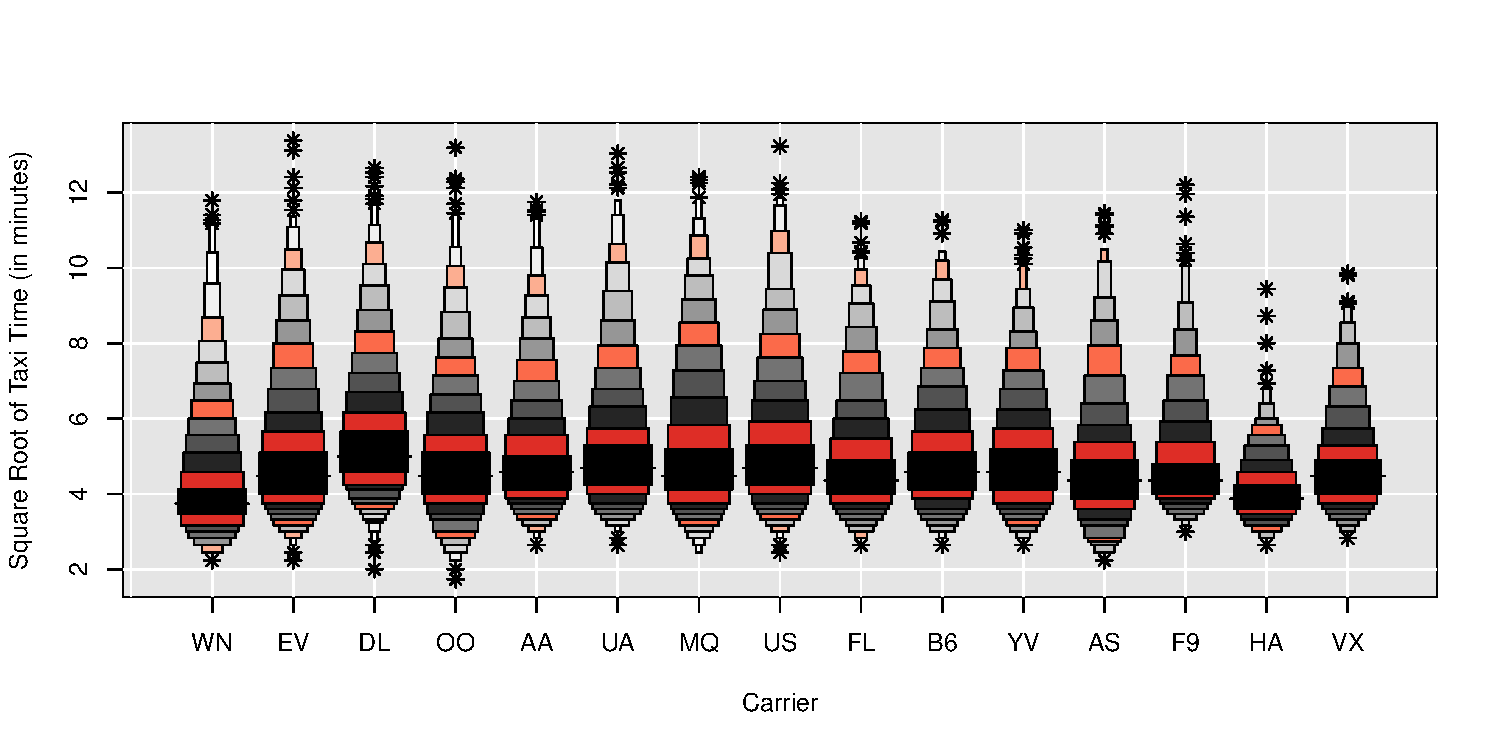
\includegraphics[width=\linewidth]{taxi-lv}

  \caption{Letter-value plots of (sqrt-transformed) taxi time for 478,755 national flights in January 2012 by airline carriers.}

  \label{fig:taxi-lv} 
\end{figure}

One consideration for letter value plots involves the number of letter values to display (i.e., when to stop displaying letter values and start showing individual observations). Figure 2 shows only those letter values whose approximate ``95\% confidence intervals'' do not overlap the successive letter values. Section~\ref{sec:extent} discusses three other rules to select the letter values based on the sample size. Some proposals for multivariate data and final discussion appears in Sections~\ref{sec:bivariate} and~\ref{sec:summary}.

Our implementation of letter-value plots is available as an R package, \texttt{lvplot}, from {\sc cran}. The online supplementary material contains all code and data used for the plots in this paper.

\section{Letter values}
\label{sec:letter-values}

Let $X_{(1)}$, ... $X_{(n)}$ denote the order statistics from a sample of size $n$. Per conventional notation, let $\lfloor y \rfloor$ and $\lceil y \rceil$ denote the largest integer below $y$ and the smallest integer above $y$, respectively. The letter values are  order statistics with specific depths, defined recursively starting with the median:
the depth of the median, $d_1$ or $d_M$, of a sample of size $n$ is defined as $d_1 = (1 + n )/2$; the depths of successive letter values (F = fourths, E = eighths, D = sixteenths, C = thirty-seconds, ...) are defined recursively as $d_i = (1 + \lfloor d_{i-1} \rfloor)/2$. We also will use the letter value itself as the subscript to the notation for depth; e.g., both $d_2$ and $d_F$ denote the depth of the fourths. 

If the depth is an integer plus $\frac{1}{2}$,  the corresponding letter value is defined as the average of the two adjacent order statistics, $X_{(\lfloor d_i \rfloor)}$ and $X_{(\lceil d_i \rceil)}$ for the lower, and similarly for the upper letter value.

The $i^{th}$ lower and upper letter values ($LV_i$) are thus defined as $L_i = X_{(d_i)}$ and $U_i = X_{(n - d_i + 1)}$. 
%The advantage of this definition for the letter values is that the median of the sampling distribution for this sample quantile from a continuous distribution $F(\cdot)$ is very close to $F^{-1} ((i - \frac{1}{3})/(n + \frac{1}{3})$, for a wide range of $F$, $n$, and $i$ \citep{dchlv}. 
Because each depth is roughly half the previous depth, the letter values approximate the quantiles corresponding to tail areas of $2^{-i}$.

The ``labeled outlier rule'' for conventional boxplots relies on the fourths because the rule is then ``unlikely to be adversely affected by extreme observations'' and ``to minimize the difficulties of masking'' \citep[pg. 992]{dchbox}. 

The breakdown point of these boxplots is 25\%; i.e., only if 25\% or more of the data values, all located in one of the tails, are contaminated, will the summary statistics and outlier identification change. This high breakdown is one of the valuable features of boxplots. In section~\ref{examples} we see that even though  letter value boxplots  perform differently in highly contaminated data, we gain a different set of valuable features.

The relatively low uncertainty in the fourths as estimates of the quartiles argues for using the fourths in the rule for labeling outliers: the standard deviation of the fourths in a Gaussian population equals roughly $[(0.25 \cdot 0.75) / (n \phi(\Phi^{-1}(0.25)))]^{1/2} \sigma$ = $1.362 \sigma / \sqrt{n}$ or a 2-SD uncertainty of roughly 0.25$\sigma$ for Gaussian samples of size 120 \citep{ha.order}. Estimates of the population quantiles beyond the quartiles, when based on order statistics, are increasingly variable; e.g., for the same $n = 120$ sample, the 2-SD uncertainty in the eighths (depth = 13) and sixteenths (depth = 7) is approximately $ 2 \times 1.607 \sigma / \sqrt{n}$ = $0.29 \sigma$ and $ 2 \times 1.968 \sigma / \sqrt{n}$ = $0.36 \sigma$, respectively. Table~\ref{tbl:letter-values} shows these factors for the standard error formula, \texttt{SEfactor}, for the first eight letter values, as well as the factor in increase in sample size needed for successive letter values to have the same uncertainty as the fourth. 
For example, the fourths in a sample of size 120 have a 2-SD uncertainty of 0.25$\sigma$; we would need a sample of size 1.4$\cdot$120 = 168 for the eighth to have this same level of uncertainty.
For small samples, then, restricting attention to estimates of only the population median and quartiles, with some general indication of the tail length beyond the quartiles, is likely to be about all the information that the data can reliably support.

\begin{table}[htpb]
  \centering
  \begin{tabular}{llr@{.}lrrr}
  \toprule
  LV & ideal tail area & \multicolumn{2}{l}{rough \%} & odds ($2^i$) & SEfactor & n-equiv*  \\
  \midrule
   M & .50 & 50 & 0\% & 2 & 1.25%3314 
   & \\
   F & .25 & 25 & 0\% & 4 & 1.36 & 1.0\\
   E & .125 & 12 & 5\% & 8 & 1.60 & 1.4\\
   D & .0625 & 6 & 25\% & 16 & 1.96 & 2.1\\
   C & .03125 & 3 & 13\% & 32 & 2.47 & 3.3\\
   B & .015625 & 1 & 56\% & 64 & 3.16 & 5.4\\
   A & .0078125 & 0 & 8\% & 128 & 4.10 & 9.1\\
   Z & .00390625 & 0 & 4\% & 256 & 5.37 & 15.6\\
%   Y & .001953125 & 0 & 2\% & 512 & 7.11 & 27.3\\
%   X & .0009765625 & 0 & 1\% & 1,024 & 9.48 & 48.4\\
%   W & .00048828125 & 0 & 05\% & 2,048 & 12.70 & 87.0\\
%   V & .000244140625 & 0 & 024\% & 4,096 & 17.11 & 157.7\\
%   U & .0001220703125 & 0 & 012\% & 8,192 & 23.14 & 288.5\\
%   T & .00006103515625 & 0 & 006\% & 16,384 & 31.40 & 531.3\\
%   S & .000030517578125 & 0 & 003\% & 32,768 & 42.75 & 984.4\\
%   R & .0000152587890625 & 0 & 0015\% & 65,536 & 58.34 & 1833.5\\
%   Q & .00000762939453125 & 0 & 0008\% & 131,072 & 79.80 & 3430.5\\
%   P & .000003814697265625 & 0 & 0004\% & 252,144 & 109.38 & 6444.3\\
%   O & .0000019073486328125 & 0 & 0002\% & 504,288 & 150.19 & 12149.2\\
%   N & .00000095367431640625 & 0 & 0001\% & 1,008,576 & 206.55 & 22977.6\\
  \bottomrule
  \end{tabular}

  \caption{First 8 letter values. Ideal \texttt{tail area} is $2 ^{-i}$, $i =
  1, ..., 8$. \texttt{rough}\% rounds $2 ^{-i} \times 100$\% to the first 1
  or 2 nonzero digits. \texttt{odds} expresses tail area as \texttt{1 in}
  $2^i$. \texttt{SEfactor} gives the factor for the asymptotic standard
  error of the order statistic (from a Gaussian population, variance
  $\sigma^2$) corresponding to \texttt{tail area}.
%  , i.e., $SE(LV) \approx$
%  \texttt{SEfactor} $\times \sigma / \sqrt{n}$, where \texttt{SEfactor} =
%  $\sqrt{p_i (1-p_i)} / \phi(\Phi^{-1}(p_i))$, $p_i$ = \texttt{tail area} =
%  $2^{-i}$. 
  \texttt{n-equiv} = (\texttt{SEfactor}/1.362633)$^2$ which gives
  the factor of increase in sample size for the uncertainty in that letter
  value to be the same as that for the fourth.
%  ; e.g., need 1.4$n$
%  (respectively, 2.1$n$) observations for the eighth (respectively, sixteenth)
%  to have the same uncertainty as that of a fourth from a sample of size $n$.
  }
  \label{tbl:letter-values}
\end{table}

% Table~\ref{tbl:counties} illustrates the letter values of the 1980 populations
% and the log populations of the 3068 counties in the continental United States.
% Along with the letter values are shown the midsummaries (average of the upper
% and lower letter values, denoted ``mids'' in Table 2), the midspreads (spread
% between the letter values, denoted ``spread''), and ``pseudo-sigma''
% \citep[pg. 40]{dchlv}, the sample letter-value spread divided by the
% theoretical letter-value spread for a standard Gaussian distribution (e.g.,
% pseudo-sigma based on the fourths is the fourth spread divided by 1.3490). For
% a symmetric population, the midsummaries should be constant, and, for a
% distribution with Gaussian-like tails, the pseudo-sigmas also should be fairly
% stable. Both the midsummaries and the pseudo-sigmas are much more nearly
% constant for the log populations than for the untransformed populations.
% 
% \begin{verbatim}
%                      Table 2
%            Letter value display for 1980
%          populations in 3068 U.S. counties
% 
%     Depth  Lower   Upper      Mid  Spread   pseudo-s
% M  1534.5  218.0   218.0   218.00     0.0     0.0000
% F   767.5  105.0   511.0   308.00   406.0   601.9365
% E   384.0   65.0  1082.0   573.50  1017.0   884.0792
% D   192.5   39.0  2280.0  1159.50  2241.0  1460.7718
% C    96.5   25.0  4572.0  2298.50  4547.0  2441.0384
% B    48.5   17.5  6641.5  3329.50  6624.0  3075.3878
% A    24.5   10.5  9694.5  4852.50  9684.0  4005.6933
% Z    12.5    8.0 14742.5  7375.25 14734.5  5539.1452
% Y     6.5    6.5 18972.5  9489.50 18966.0  6572.5570
% X     3.5    4.5 38316.0 19160.25 38311.5 12369.4452
% W     2.0    4.0 70716.0 35360.00 70712.0 21446.1187
% V     1.5    2.5 72745.5 36374.00 72743.0 20860.5759
% U     1.0    1.0 74775.0 37388.00 74774.0 20383.6663
% 
%              Letter value display for 1980
%          log populations in 3068 U.S. counties
% 
%     Depth  Lower   Upper      Mid  Spread   pseudo-s
% M  1534.5 2.3385  2.3385   2.3385  0.0000     0.0000
% F   767.5 2.0212  2.7084   2.3648  0.6872     1.0189
% E   384.0 1.8129  3.0342   2.4236  1.2213     1.0617
% D   192.5 1.5911  3.3579   2.4745  1.7669     1.1517
% C    96.5 1.3979  3.6601   2.5290  2.2622     1.2144
% B    48.5 1.2429  3.8223   2.5326  2.5794     1.1976
% A    24.5 1.0207  3.9865   2.5036  2.9658     1.2268
% Z    12.5 0.9031  4.1685   2.5358  3.2654     1.2276
% Y     6.5 0.8116  4.2780   2.5448  3.4664     1.2013
% X     3.5 0.6505  4.5512   2.6009  3.9007     1.2594
% W     2.0 0.6021  4.8495   2.7258  4.2475     1.2882
% V     1.5 0.3010  4.8616   2.5813  4.5606     1.3078
% U     1.0 0.0000  4.8738   2.4369  4.8738     1.3286
% \end{verbatim}

Letter values are particularly useful for large data sets, because (a) much of the most valuable information, especially for inference purposes, is contained in the tails (cf.\ Winsor's principle, ``All distributions are normal in the middle'' \citep[pg. 457]{tukey60}); and (b) adjacent letter values have asymptotic correlation $\sqrt{1/2}$ = 0.707 (\citet{mosteller46} cited by \citet[pg. 51--52]{dchlv}). Thus, rather little information concerning tail behavior is lost by considering only the letter values. 
%Figure~\ref{qqpop4} illustrates this retention of tail information in visualizing the distribution of the 1980 populations and their logarithms in 3068 continental U.S. counties via normal quantile-quantile (QQ) plots (panels A and B, respectively) versus using only the 25 letter values (panels C and D, respectively); the right column reveals the advantage of logarithms.

%\begin{figure}[hbtp]
%  \centering
%  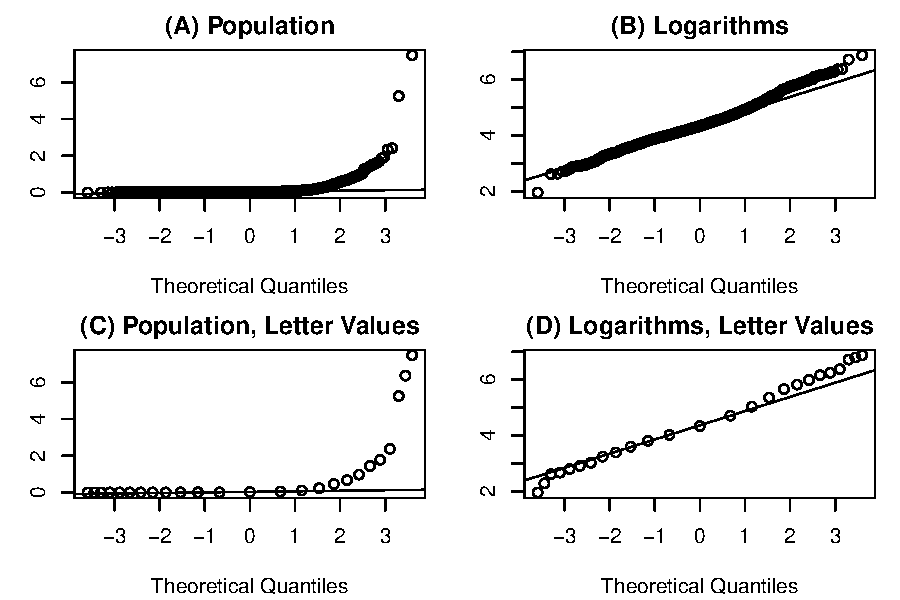
\includegraphics[width = 0.75 \linewidth]{counties-qq}
%
%  \caption{QQ plots on 3068 Continental U.S. county populations (A) and their
%  logarithms (B), versus QQ plots (C), (D) using only 25 letter values.}
%  \label{qqpop4}
%\end{figure}

\section{Letter-value plots}
\label{sec:lv-boxplots}

Letter-value plots are based on the letter values, with one box for each pair of lower and upper letter values. The median is shown by a vertical line segment, and the innermost box is drawn at the lower and upper fourths, as in the conventional boxplot. An incrementally narrower box is drawn between at the lower and upper eighths, and narrower one still at the lower and upper sixteenths. We continue in this fashion until we reach a box that corresponds to a stopping rule described in the following section. Boxes with matching heights (for horizontally drawn plots) correspond to the same depths. We also shade more heavily the innermost boxes, to indicate a higher data density. The use of color stripes, as shown in figure~\ref{fig:taxi-lv} also helps with identifying corresponding boxes across different plots.

Beyond the most extreme box, all observations are identified individually. With this definition, the expected proportion of the outliers (roughly $1/2^i$) equals the expected proportion between this end and the end of the next bigger box (i.e., roughly $1/2^{i-1} - 1/2^i$ = $(1/2^{i-1})(1 - 2^{-1})$ = $1 / 2^i$). When the depth, $d_i$, reaches 1, the letter values are the extremes (minimum and maximum).

Letter-value plots for three different distributions are shown in Figure~\ref{stackbox}. Each panel displays a sample of 10,000 data points (top = standard Gaussian, middle = exponential with mean 1, bottom = standard uniform), first using the proposed letter-value plot up to letter Y, corresponding roughly to tail area $2^{-9}$ = 1/512 (top row), and then with the the conventional boxplot (bottom row). Comparing the left (Gaussian) and right (Uniform) letter-value plot, overall \textit{more heavily shaded} displays correspond to distributions with \textit{lighter} tails. This phenomenon is shown more forcefully in Figure~\ref{t-dist} which shows three decreasingly heavy-tailed $t$ distributions with 2, 3, and 9 degrees of freedom.

\begin{figure}[hbtp]
  \centering
  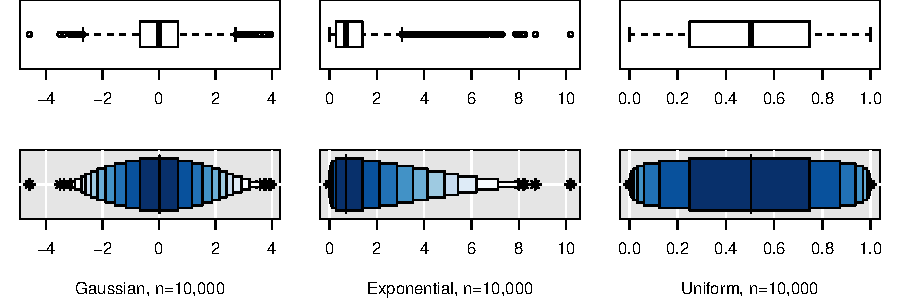
\includegraphics[width = \linewidth]{boxplots}

  \caption{Letter-value plots (top row) and standard boxplots (bottom row) for
  data from three different distributions. Each plot shows 10,000 data points.
  From left to right, samples come from $\mbox{N}(0,1)$, $\mbox{Exp}(1)$, and
  $\mbox{U}[0,1]$. }

  \label{stackbox}
\end{figure}

\begin{figure}[hbtp]
  \centering
  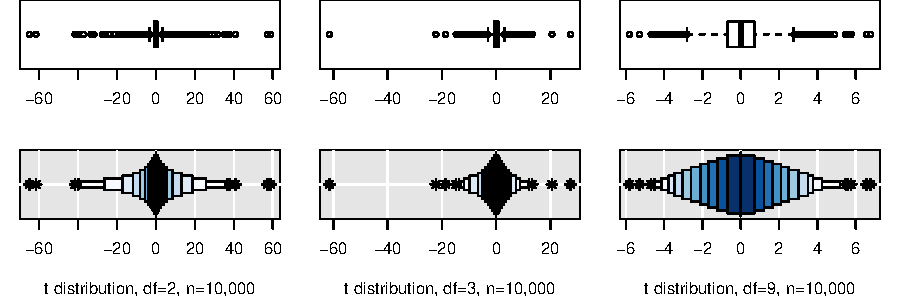
\includegraphics[width = \linewidth]{t-dist}
  
  \caption{Letter-value plots and standard boxplots for samples of 10,000
  for $t$ distributions on 2, 3, 9 degrees of freedom. Top row: Letter-value
  plots. Bottom row: Conventional boxplots.}
  \label{t-dist}
\end{figure}

Figure~\ref{lvpops} shows letter-value plots and boxplots for the 1980 populations and log populations of the 3068 counties in the United States. While the skewness in the distribution of the populations is evident from both the letter-value plot and the conventional boxplot, the former shows more clearly that the right tail of the log populations above the median is somewhat more extended than the left tail below the median (i.e., the boxes to the right of the median are slightly longer than those to the left of the median).

\begin{figure}[hbtp]
  \centering
  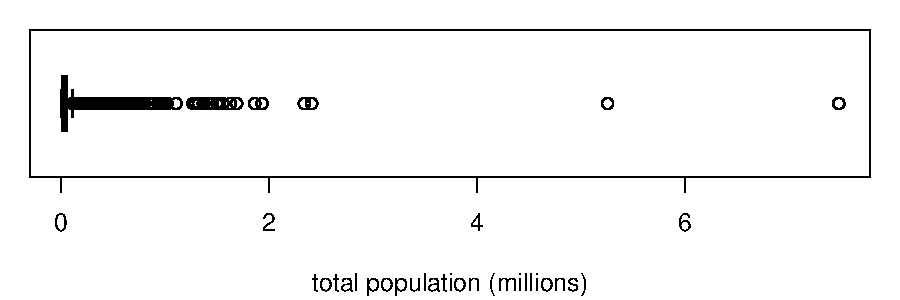
\includegraphics[scale=.5]{counties-lvpop-a.pdf}
  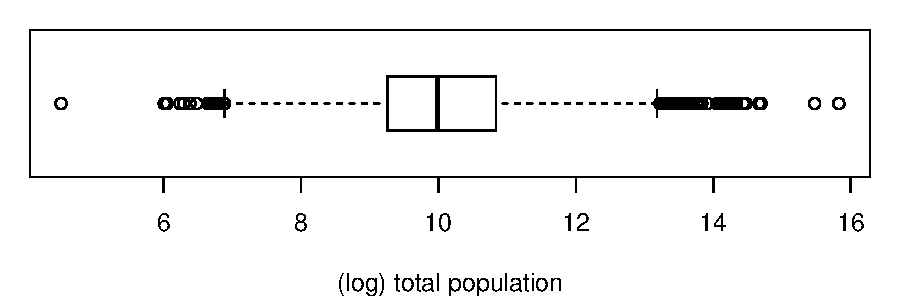
\includegraphics[scale=.5]{counties-lvpop-c.pdf}
  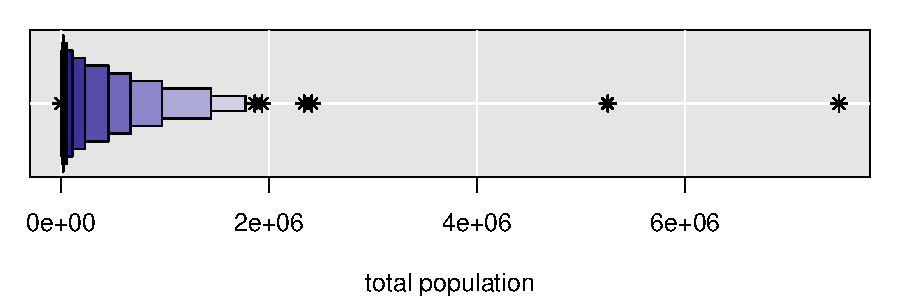
\includegraphics[scale=.5]{counties-lvpop-b.pdf}
  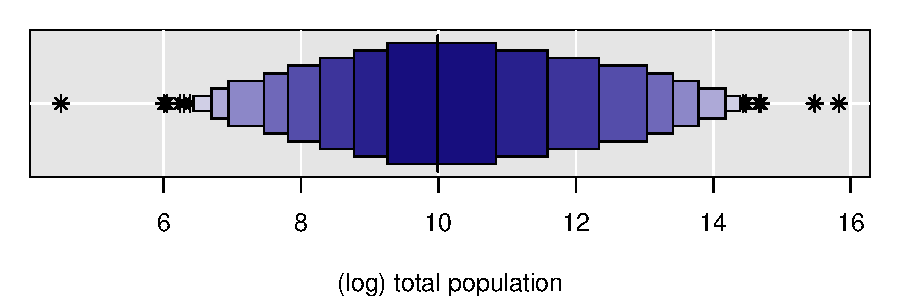
\includegraphics[scale=.5]{counties-lvpop-d.pdf}
 
  \caption{Letter-value plots and standard boxplots for the 1980
  populations and log populations of 3068 counties in the continental United
  States.}
  \label{lvpops} 
\end{figure}

%\section{Extent of letter-value plots}
\section{How far out? -- Stopping rules}
\label{sec:extent}

We need a rule to determine the number of boxes to show in a letter-value plot, which will determine the number of labeled outliers. In this section, we consider four proposals for such a rule. The first two rules are based on using a constant -- either absolute or relative to sample size; the second two rules are based on `trustworthiness'  and make use of the standard error of the letter values involved:
\begin{enumerate}
\item[(i)]{\bf Rule 5--8:}
we can choose the extent of the letter-value plot display so that the last set of boxes encompasses all but the 5--8 most extreme observations, if we stop the letter-value plot display at $LV_k$ where 
%
\begin{equation}
k = \lfloor \log_2 n \rfloor - 3.
\end{equation}
%

\noindent Tukey identified 5--8 extreme points  in many of the displays in \textit{Exploratory Data Analysis}.
%, since 
%Recall that the depth of the $k^{th}$ letter value, $d_k$, is defined in terms of the previous depth: $d_k = (1 + \lfloor d_{k-1} \rfloor)/2$, which implies that $2 d_{k} -1 \leq d_{k-1} \leq 2 d_k - (1/2)$. 

\item[(ii)]{\bf Constant percentage:}
an alternative criterion fixes the number of labeled outliers as a percentage of the overall sample size.
 Let $p$ denote this proportion, the last set of boxes to be drawn ends with depths

\begin{equation}
k(p) = \lfloor \log_2 n \rfloor - \lfloor \log_2 (np) \rfloor + 1
\end{equation}

\noindent In effect, conventional boxplots use this rule, with $p = 0.007$. This criterion results in the same rule as the previous rule for the samples in Figure~\ref{stackbox} ($n = 10,000$) when $p$ lies between 0.004 and 0.006 (0.4--0.6\%), and in Figure~\ref{lvpops} ($n = 3068$) when $p$ lies between 0.011 and 0.020 (1.1--2.0\%).

\item[(iii)] {\bf  `Trustworthiness':}
to assess the ``trustworthiness'' of the $k^{th}$ letter value we interpret the values as an estimate of the corresponding population quantile. We can ``trust''  a given letter value, if  its approximate 95\% confidence does not overlap the subsequent letter value.

Since a letter value can be viewed as the median between the extreme and the previous letter value, we can express an approximate $1-\alpha$ confidence interval for the median of $m$ values (with $m > 10$) as approximately $0.5 \sqrt{m} z_{1-\alpha/2}$ observations on both sides of the sample median (rounding to the nearest integer), where $z_{1-\alpha/2}$ is the ${1-\alpha/2}$ quantile of a standard Gaussian distribution (\citet[161]{ha.order}. This approximation is based on the Gaussian approximation to the binomial distribution; it leads to a straightforward rule for $k$ given as:
\begin{equation}
k(1-\alpha/2) =  \left \lfloor \log_2 (n) - \log_2 
   \left(2  z_{1-\alpha/2}^2 \right) \right \rfloor + 1
\end{equation}
see below for a proof.
\item[(iv)]{\bf Maximal standard error}:
this fourth rule gives us the maximum letter value, for which the standard error is fixed to be below a relative upper limit. 

For a sample from a Normal distribution, the asymptotic standard error is given as 
\begin{equation}
SE(LV_i) \approx \sigma \sqrt{p_i \cdot (1 - p_i)/ n} / \phi(\Phi^{-1}(p_i)) 
 = (SEfactor) \sigma / \sqrt{n},
\label{SELV}
\end{equation}
where $p_i = 2^{-i}$, $i = 1, ..., \log_2n$.
As sample size $n$ increases, we can increase the number of letter values shown while keeping the same standard error. Figure \ref{fig:lv-error} gives an overview of  the situation.




%\noindent When $i = 2$ ($p_i = 0.25$, fourths) and $n = 120$, this standard error is approximately 0.125$\sigma$; when $n = 186$, it is 0.10$\sigma$, and when $n = 743$, it is 0.05$\sigma$. Thus, a rough 2-SE interval around the fourth is roughly 0.25$\sigma$, 0.2$\sigma$, or 0.1$\sigma$, respectively, as $n$ increases from 120 to 186 to 743. How many more letter values can be shown with the same level of uncertainty when $n$ increases? For illustration, consider only the last (and most stringent) criterion, where 2$SE$ $\approx$ 0.1$\sigma$. If $n \geq 1032$, the asymptotic 2-SE uncertainty in $LV_3$, the eighth (E), using the formula in (\ref{SELV}), does not exceed 0.1$\sigma$. For the same precision in $LV_4$ (sixteenth), one needs $n \geq 1550$.

\end{enumerate}





\begin{proof} for (iii):
Consider the upper $k^{th}$ letter value, $LV_k$. If its upper 95\% confidence limit does not extend beyond the next letter value, $LV_{k+1}$, we continue to the next letter value, $LV_{k+1}$; otherwise, the box corresponding to $LV_k$ is the last box shown. Since approximately $d_{k+1}$ observations lie between $LV_k$ and $LV_{k+1}$, and the upper 95\% limit for $LV_k$ has roughly $\sqrt{d_{k-1}} \approx \sqrt{2 d_k }$ observations, this principle requires $\sqrt{2 d_k} < d_{k+1} \approx d_k / 2$, or $d_k > 8$. A rule such as this one with 95\% confidence level often leads to labeling 5--8 of the most extreme observations on each side, surprisingly consistent with many of the displays in \citet{eda}.
\end{proof}



\noindent The third stopping rule has the obvious advantage that it provides a simple, distribution-free solution. Neither the overall sample size, nor any distribution-related characteristic such as skewness or kurtosis, affects the rule. When $\alpha = 0.05$ (95\% point-wise confidence), the rule leads to showing only those letter values whose depths are at least 10 (i.e., labeling 5--8 observations on each side). Because the first rule is a special case of this third rule, we will consider the use of only stopping rules 2 and 3. Note that $k = 7$ when $n$ is between 492 and 983, which corresponds to letter value A (Gaussian tail area 0.78\%). When $n$ is between 984 and 1966, $k = 8$, corresponding to letter value Z (Gaussian tail area 0.39\%), which is very close to the expected percentage of outliers from a Gaussian sample that are labeled by the conventional boxplot rule (Gaussian tail area 0.35\%).

% KK: I think we need more discussion about the differences 
% between rules 2 and 3, esp since they give diff answers
% depending on $p$.  I also think we'd better number those 2 eqns 
% for later reference.


\begin{figure}[hbtp]
  \centering
  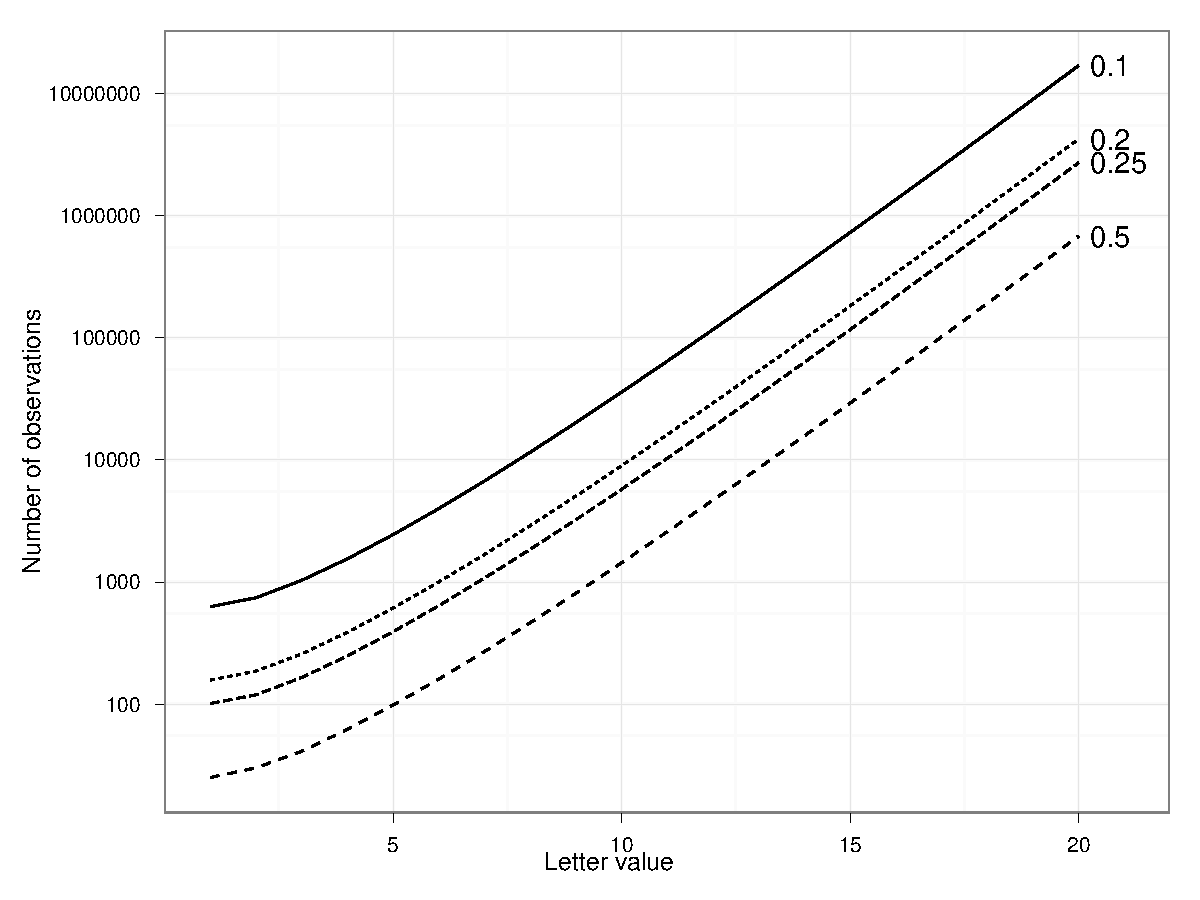
\includegraphics[width=0.65\linewidth]{letter-val-errors}

  \caption{Plot of letter value vs. number of observations (on log-scale) needed for a 2-SD uncertainty of no more than 0.50, 0.25, 0.20 and 0.10 $\sigma$. }
  \label{fig:lv-error} 
\end{figure}

The different rules provide the user with choices depending on the desired precision in the letter values shown. Our current implementation of the letter-value plot display uses rule 3 as a default.

\section{Examples}
This first example demonstrates the behavior of letter value boxplots in situations with contaminated -- or rather -- heterogenous data.
The plots in figure \ref{fig:xpl:histogram} give an overview of the situation: to  standard normal random samples of size $n= 1,500$ a set of points from a normal distribution $N(4,1)$ are added, starting with 1\% contamination (of the original sample size $n$), ending with 30\%, which is resulting in an essentially bimodal distribution. Figures \ref{fig:xpl:boxplot} and \ref{fig:xpl:lvplot} show a comparison of boxplots versus letter value plots.  
\begin{figure}[htbp] %  figure placement: here, top, bottom, or page
   \centering
   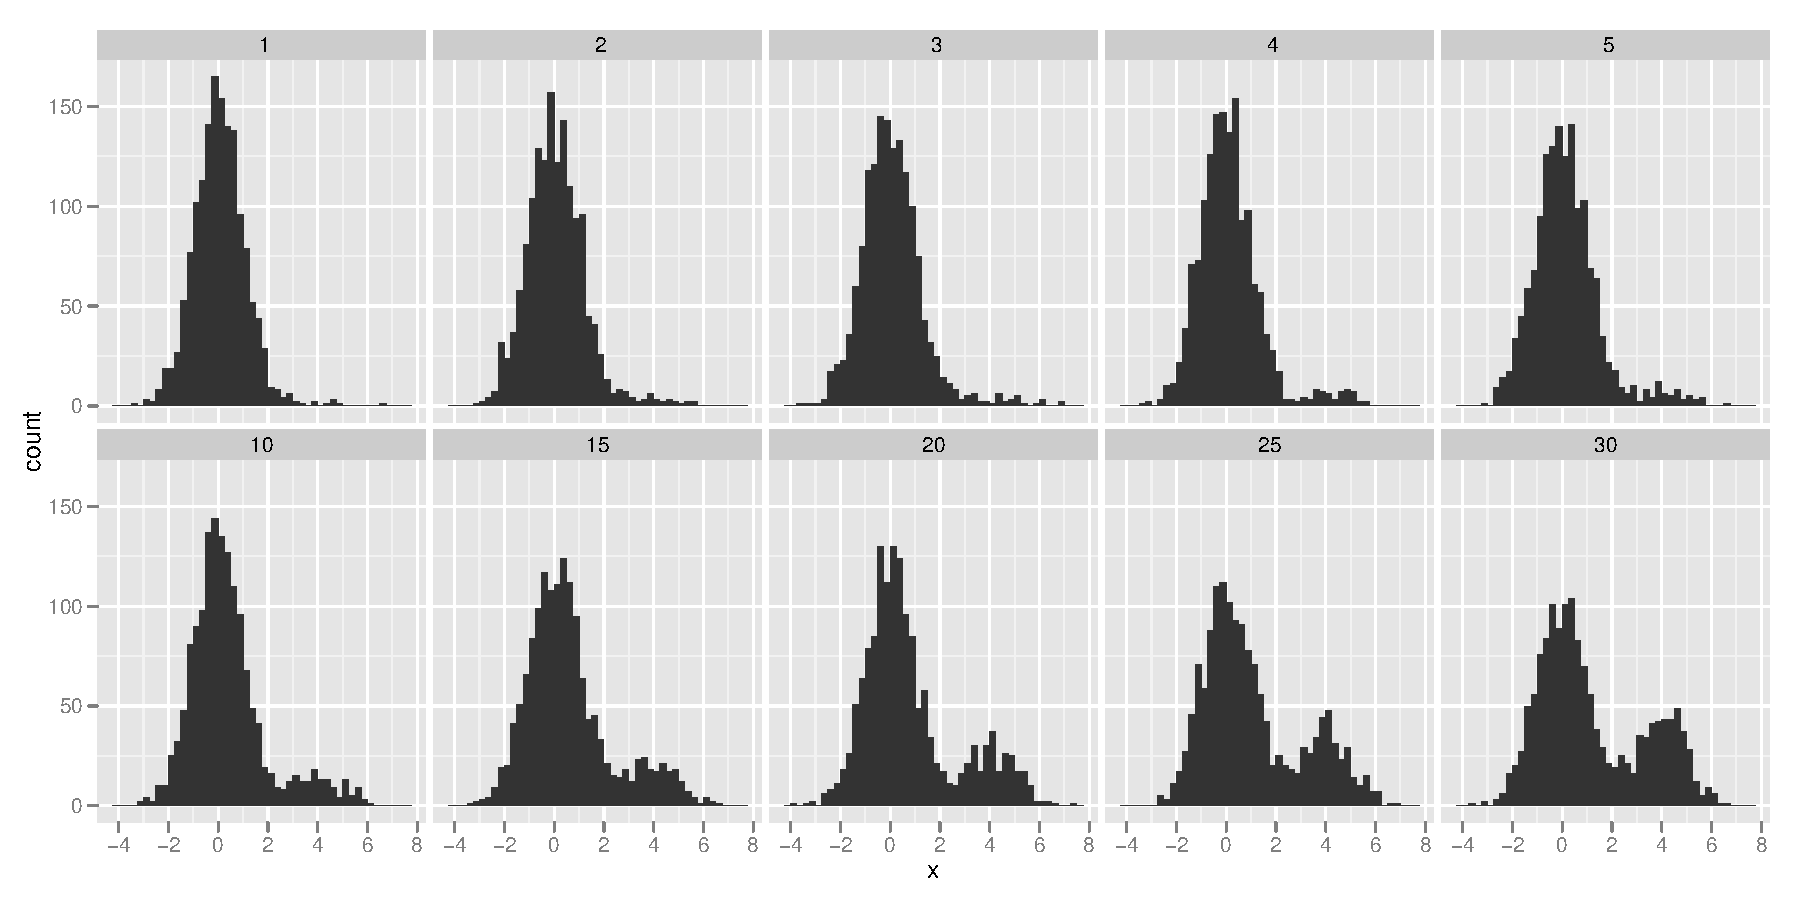
\includegraphics[width=.9\linewidth]{xpl-histogram} 
   \caption{Histograms as an overview of the bi-modal samples resulting from contaminating a sample from a standard normal distribution with samples from $N(4,1)$.}
   \label{fig:xpl:histogram}
\end{figure}

In the boxplots, we see that up to 5\% of contamination in the upper tail area is going by the boxplots unnoticed.  Up to 20\% of contamination raises the median slightly and increases the inter-quartile range some at the cost of some of the outliers. Beyond 25\% the number of outliers becomes a lot smaller, while the upper whisker is extended to beyond the second mode and the upper quartile is raised. 
The letter value plots are more sensitive - and thereby are able to give a better summary of the actual underlying distribution.
With 1\% of contamination (that is fifteen additional points from a normal distribution with mean 4), we see that the  three outmost letter values are shifted upward - indicating an asymmetry in the data, that is restricted to the outer tail area. As the percentage of contaminated points gets higher, letter values at a higher depth are affected. For 30\% contamination, we see that the upper eighth is shifted into the mean of the second mode. 
\begin{figure}[htbp] %  figure placement: here, top, bottom, or page
   \centering
   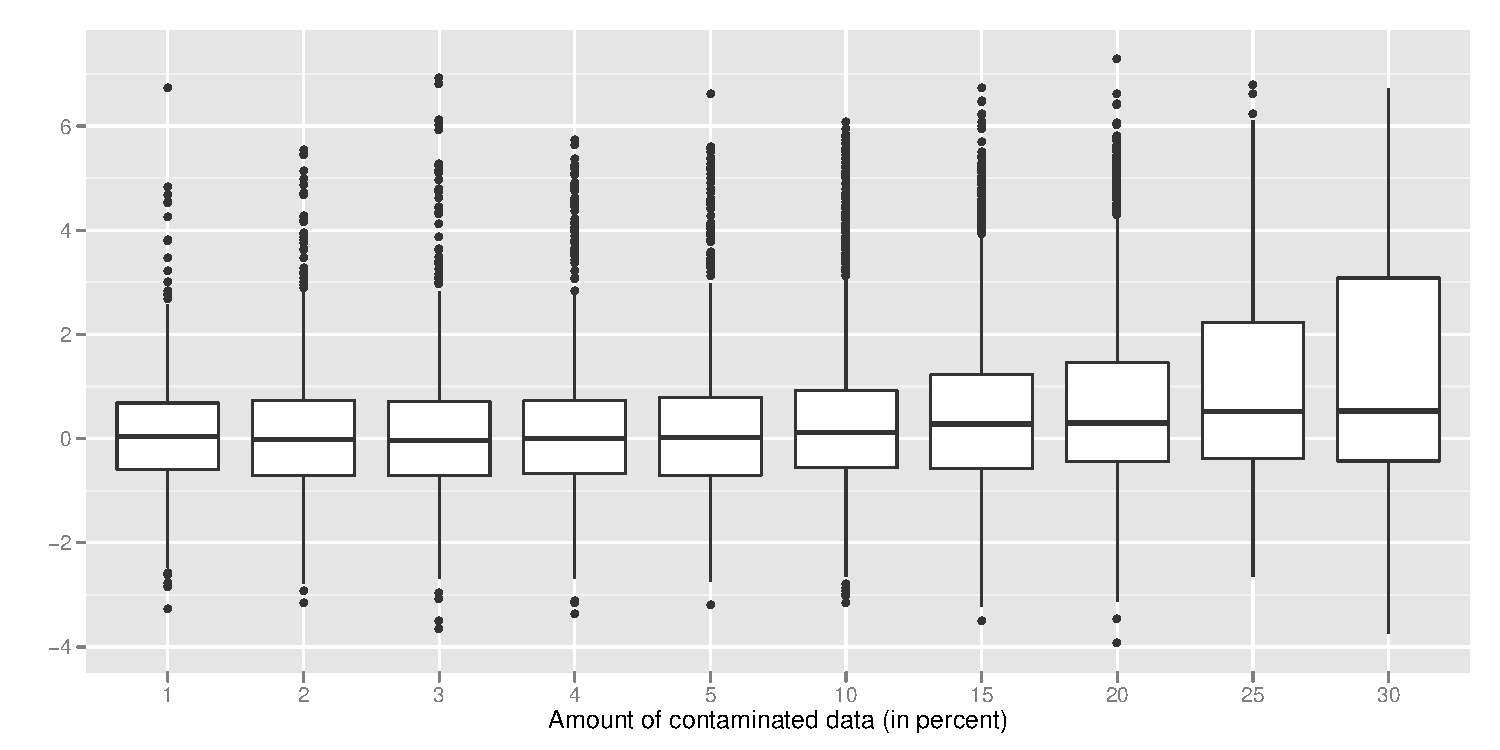
\includegraphics[width=.8\linewidth]{xpl-boxplot} 
   \caption{Boxplots of contaminated data. Boxplots are robust towards contamination of less than 25\%.}
   \label{fig:xpl:boxplot}
\end{figure}

\begin{figure}[htbp] %  figure placement: here, top, bottom, or page
   \centering
   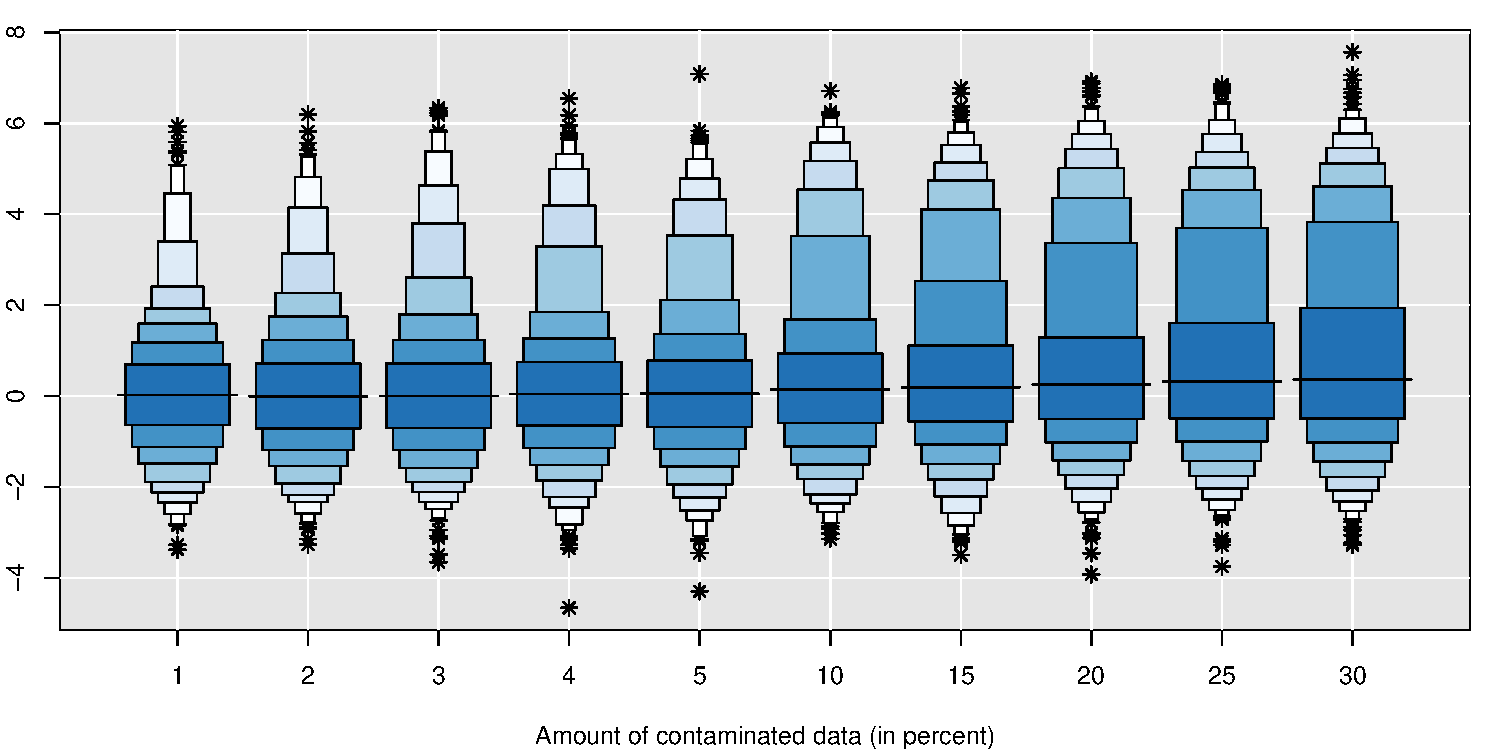
\includegraphics[width=.8\linewidth]{xpl-lvplot} 
   \caption{Letter value plots of contaminated data. Even small contaminations in the data can be seen in the outermost letter values - indicating changes from a standard normal situation. As the contamination becomes larger, more of the inner letter values are reacting to the changes, allowing pinpointing as to where the source of the contamination sits.}
   \label{fig:xpl:lvplot}
\end{figure}

\begin{figure}[htbp] %  figure placement: here, top, bottom, or page
   \centering
   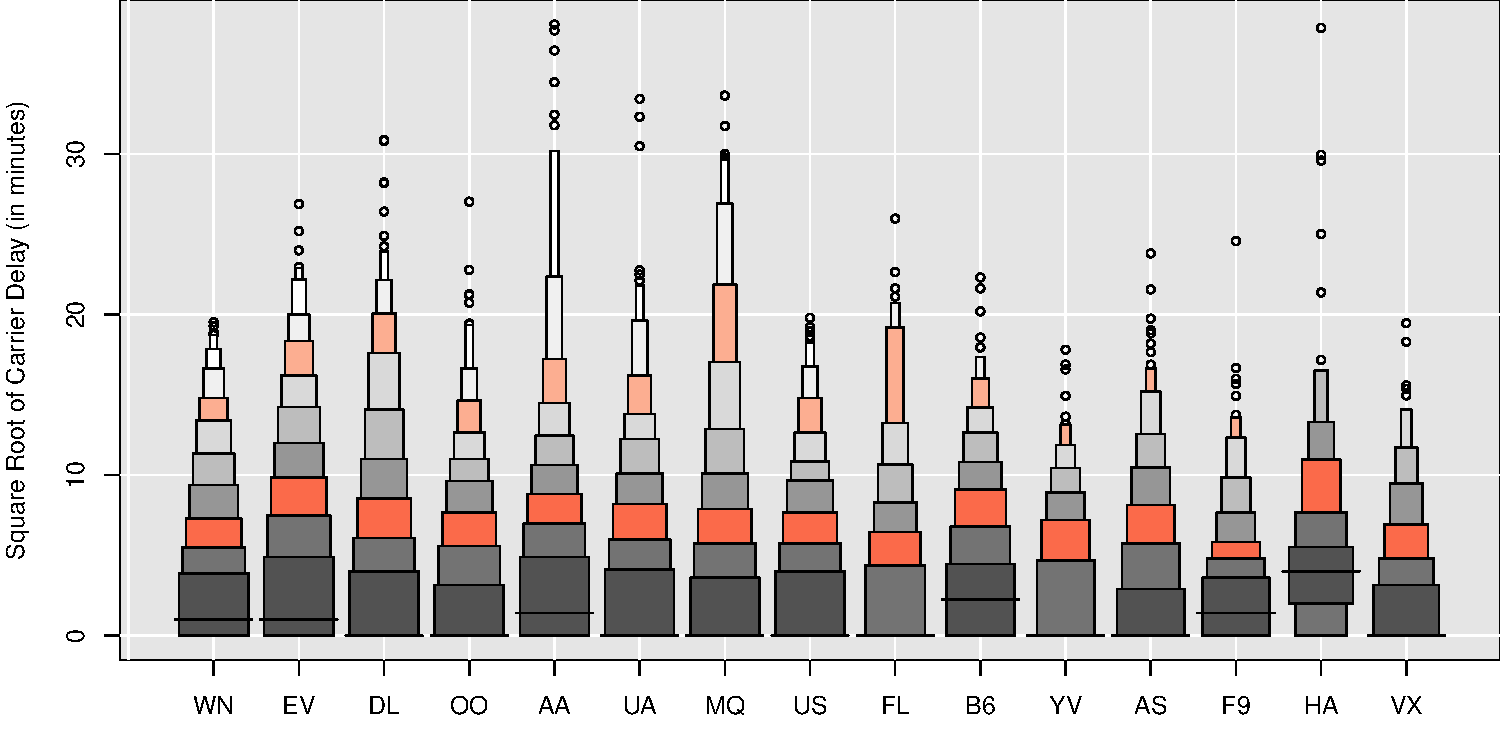
\includegraphics[width=.8\linewidth]{carrier-lv} 
   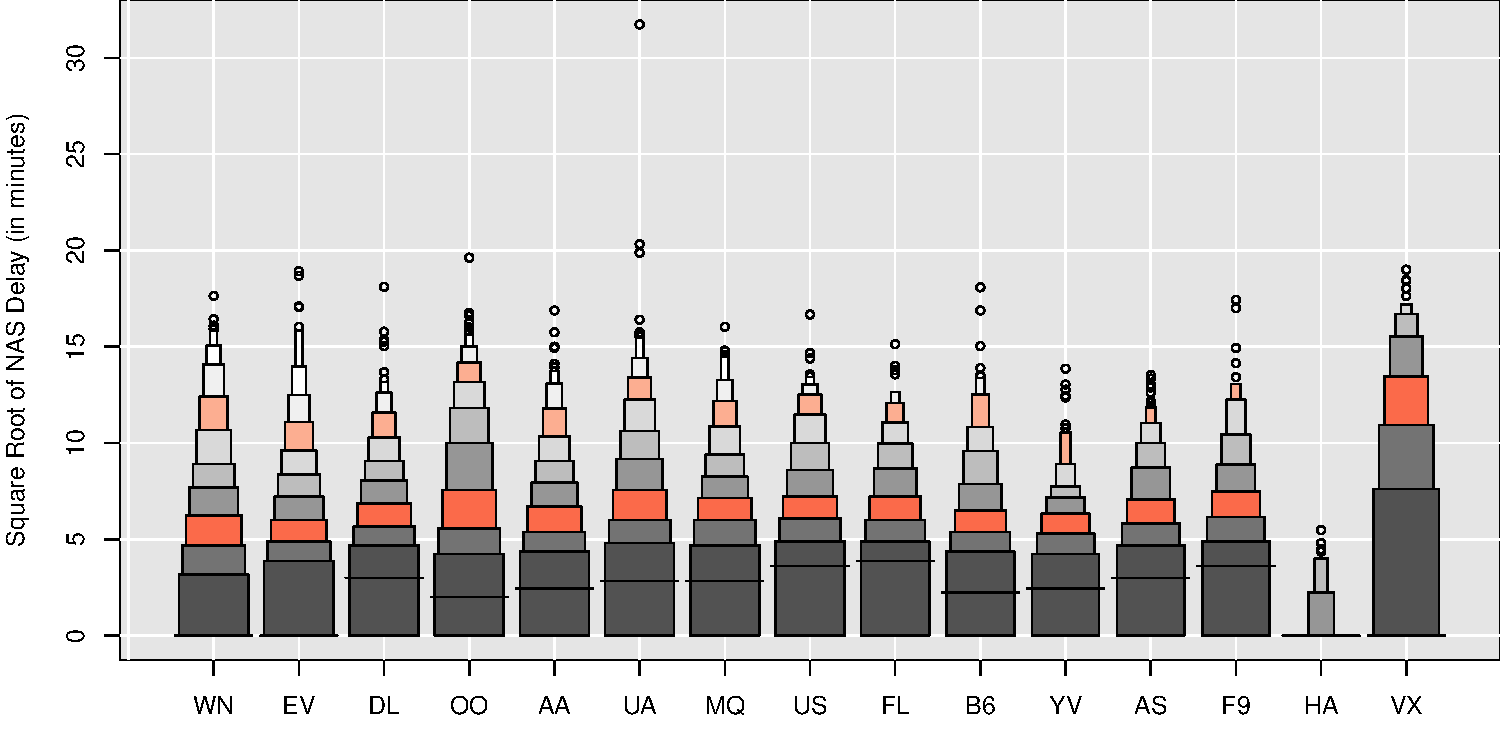
\includegraphics[width=.8\linewidth]{nas-lv} 
   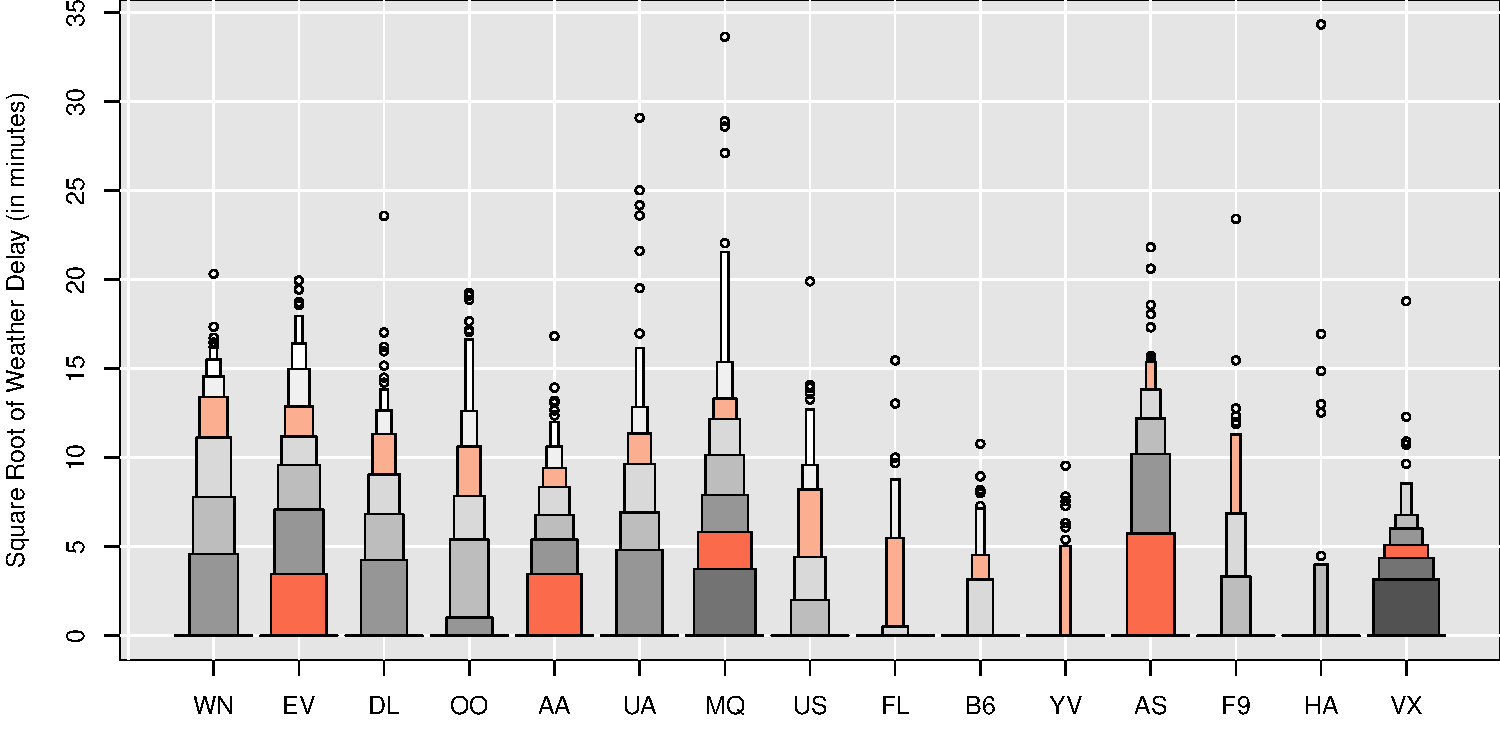
\includegraphics[width=.8\linewidth]{weather-lv} 
   \caption{Letter value plots of different types of delays by airline carriers: carrier delay (top), NAS delays (middle), and weather related delays (bottom). }
   \label{fig:xpl:delays}
\end{figure}


The second example shows again an aspect of flight data: figure \ref{fig:xpl:delays} displays all 70,908 delayed flights in January 2012. As soon as a flights is delayed, FAA guidelines require airline carriers to report a reason for the delay. The three most common reasons for delays are inclement weather, carrier delays, and National airport security (NAS). While the different sources of delay have to be stated,  delays of  less than15 minutes can be reported as zero, leading to highly zero-inflated  distributions for these types of delays. Zero-inflations lead to letter value boxplots that are seemingly `cut off' -- indicating that a lot of the lower letter values coincide. From the letter value boxplots in the top row of figure~\ref{fig:xpl:delays} we see that most airline carriers have median delay times due to carrier delays close to zero, with the notable exception of Hawaiian Airlines (HA), where the median delay is close to 25=5$^2$ minutes, even though this carrier is one of the smallest, it shows some of the most extreme delays, indicating a potential organizational problem.
Not surprisingly, all airline carriers seem to be affected similarly by delays due to National Airline Security (NAS), as we can see from the letter value boxplots in the middle of figure ~\ref{fig:xpl:delays}. The two exceptions are the two smallest airline carriers: again, Hawaiian Airlines are an exception -- there are almost no problems due to NAS delays, whereas Virgin America  (VX) seems to be affected by NAS delays often and long.
Weather delays, as shown in the bottom row of figure~\ref{fig:xpl:delays} affect different airline carriers differently, due to different routes serviced. Haiwaiian Airlines (HA) is not likely to be affected by inclement weather in January, and therefore delays due to weather are minimal, with the exception of six very large outliers. Virgin America, on the other side is affected the most by weather delays.


\section{Bivariate letter value plots}
\label{sec:bivariate}

\citet{bagplots} proposed the ``bagplot'' as a two-dimensional version of the boxplot, using location depths (introduced by \citet{tukey75}) to define analogues of the median and fourths, and then connecting the points corresponding to the fourth-depths via linear segments. 

The location depth $ldepth(p,Z)$ is defined for an arbitrary point $p \in \Reals^2$, relative to a set of $n$ points $Z$ = \{$z_i = (x_i, y_i)$, $i = 1,...,n$\}, as the smallest number of $z_i$'s contained in any closed halfplane with boundary line through $p$. That is, if one were to pass a line in the plane through $p$ and keep track of the smaller of the two numbers of $z_i$ on either side of the line as the line is rotated through every angle to its opposite side ($180^o$), then the location depth of that point $p$ relative to $Z$ is the smallest of all the numbers. The analog of the one-dimension median in two dimensions using location depth would thus be that point $p_M$ for which $ldepth(p_M, Z)$ is largest (e.g., $n/2$). If such a $p$ is not unique, then the ``depth median'' is defined as the ``center of gravity'' of all points $p$ for which $ldepth(p,Z)$ is largest. Recall that a property of the fourths for a univariate sample is that the interval between the lower and upper fourth contains one-half of the data. Thus, an analog of the box for the bagplot was defined as the convex hull of all points $p$ for which $ldepth(p,Z) \ge 1 +  \lfloor 0.5 \cdot  ldepth(p_M, Z) \rfloor$. Similarly,  successive letter areas are defined based purely on their depth as the convex hull of all points in the sample with $ldepth_i(p,Z) \ge 1 +  \lfloor 0.5 \cdot  ldepth_{i-1}(p, Z) \rfloor$.
Figure~\ref{counties-bag} shows a side-by side comparison of a standard bagplot (left, \citet{bagplots}, implemented in \citet{aplpack}) of average temperatures in January by degree latitude of each of 3,068 US counties and a letter-value bagplot on the right.
The asymmetry of the bivariate display around the principal axis,
and the cluster of points above the upper right edge of the final contour,
are much more evident in the letter value bagplot.  All of these points correspond to counties along the West Coast of the United States, the state of Washington, some counties in the northern part of Oregon and some in the East of Montana.

%%% KK: HW or HH: can you identify those points?
%%% KK: single sentence should not be a paragraph on its own; add to former.
Algorithms for fast computation of bivariate letter values for a bivariate letter-value plot are currently under development.

\begin{figure}[hbtp]
  \centering
  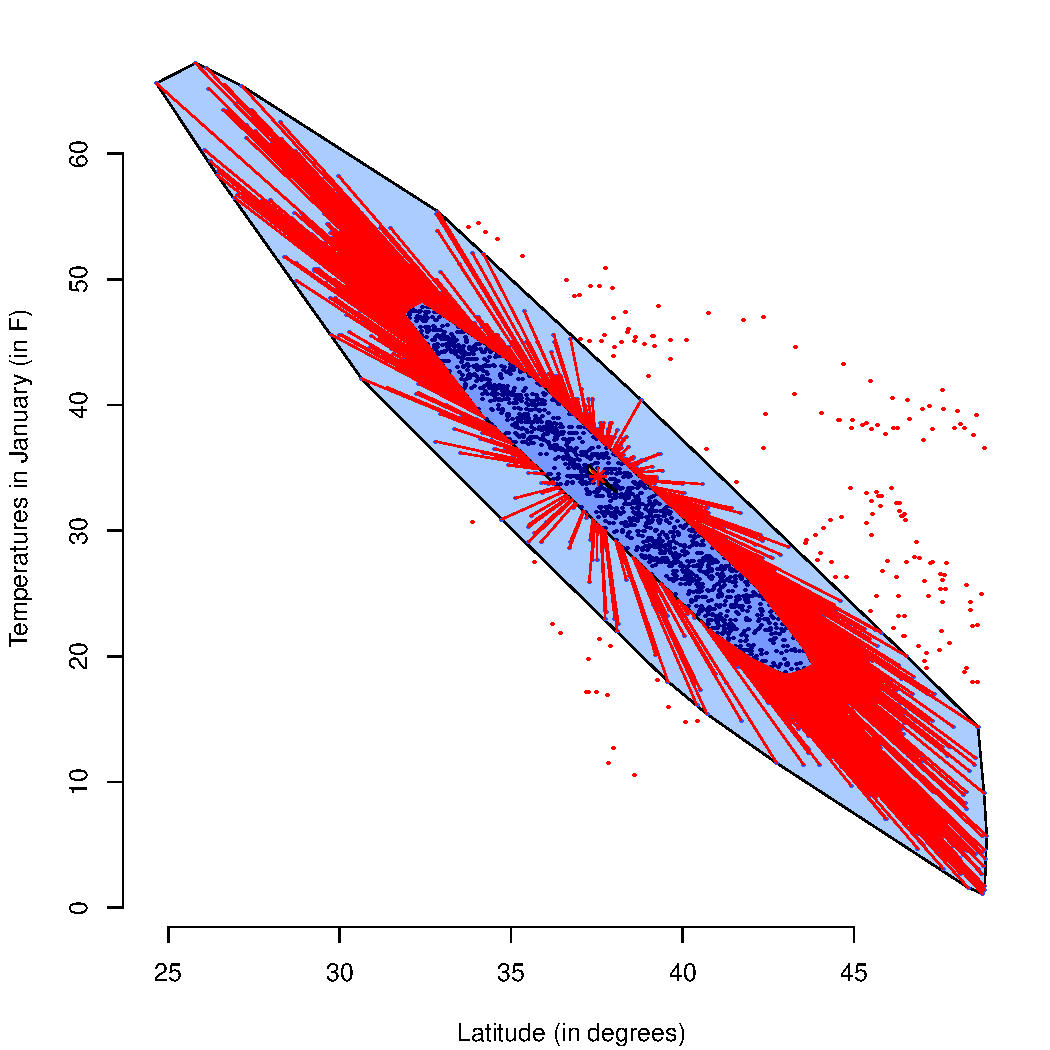
\includegraphics[width=0.5\linewidth]{images/counties-bag}%
  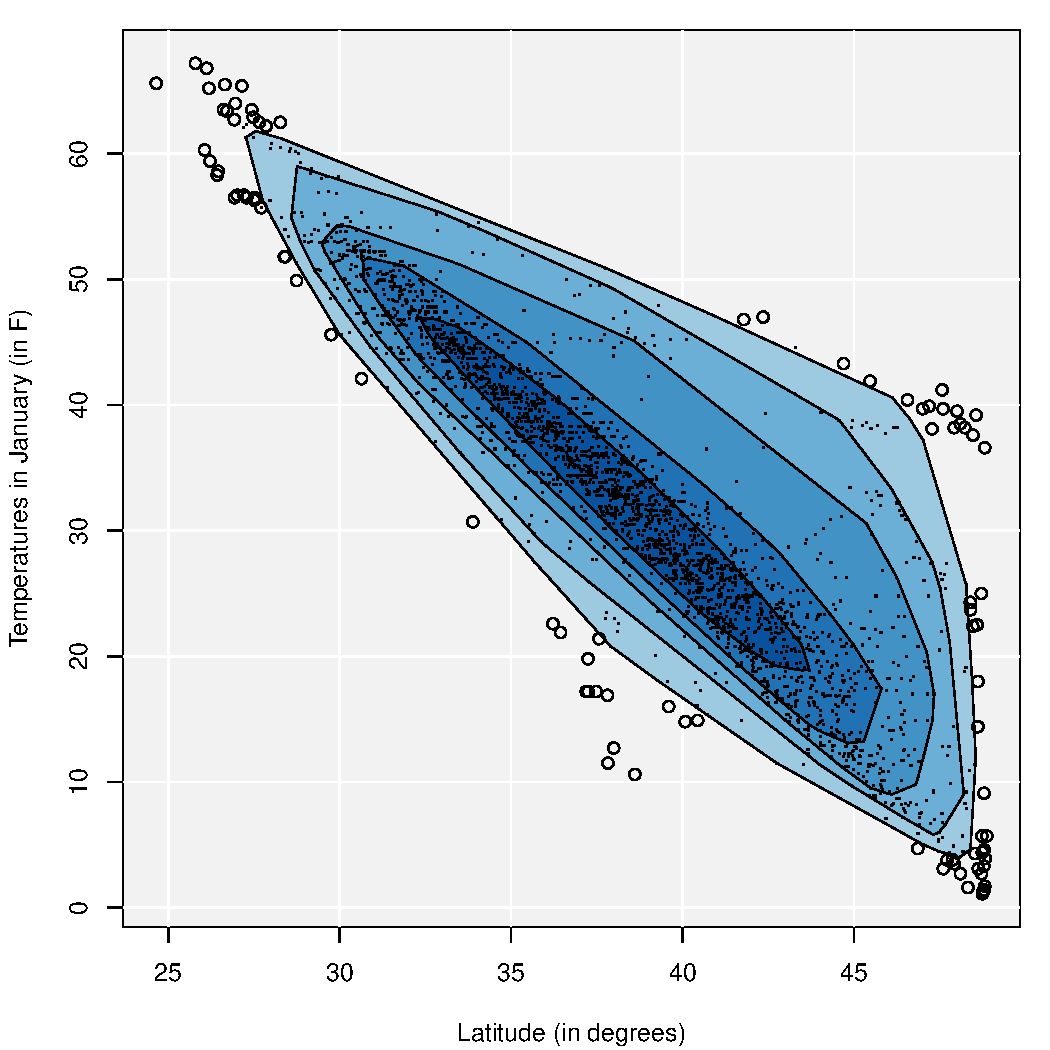
\includegraphics[width=0.5\linewidth]{images/counties-lvbag}

  \caption{Bagplot (left) and letter-value bagplot (right) of average January
  temperatures by degree latitude for 3,068 US counties. }

  \label{counties-bag} 

\end{figure}

\section{Summary}
\label{sec:summary}

Letter-value plots provide a natural extension of boxplots in situations where we are dealing with large amounts of data. Like boxplots, they show only actual data values, rather than smoothed values or estimated densities. Letter-value plots convey further information about tail behavior beyond the whiskers. Simple stopping rules that depend on neither the number of points nor on their distribution, allow us to construct reliable plots that are less prone to over-interpretation when dealing with small number of points: Rule 3 will ensure that a box for quartiles is drawn only if there are at least 16 data points. This rule is sensible in situations where we are dealing with groups of very different sizes, such as Figure~\ref{fig:internet-lbp}. Additionally, for large data situations, fewer observations will be labeled as as outliers compared to a conventional boxplot, where there is a fixed rate of outliers -- for a normal distribution it is approximately 0.7\%. Letter values can be extended to two dimensions by using the location depth, giving rise to letter-value bagplots as a two dimensional extension of letter-value plots, and providing a robust, data-based assessment of data concentration in two dimensions. Implementation details are found in the online supplementary material.

%%%% KK: 16 data points??? would you trust an eighth in a sample of only n=16?
%%%% Presumably it should be much more?


%The advantages of the letter value boxplot are:
%
%\begin{itemize}
%\item they are based on actual data values 
%\item they are simple to compute from the letter value display
%\item they convey further information about tail behavior beyond the whiskers
%\item for large data sets, fewer observations are labeled as ``outliers'' 
%compared to a conventional boxplot (roughly 0.7\%)
%\item their construction does not depend on a smoothing parameter.
%\end{itemize} 

% \appendix
% \section{Implementation}
% 
% The Appendix contains the R code for implementing these letter-value boxplots. The code has been posted also on \texttt{http://statlib.cmu.edu}. Further information about the code and its implementation are available from the first author.
% 
% \begin{verbatim}
% LVboxplot <- function(x, k = NULL, perc = NULL, alpha = 0.95, horizontal = T,
%   col = T, ...) 
% \end{verbatim}
% 
% \begin{itemize}
% \item[x] vector of data values to be displayed
% \item[k] number of letter-value statistics shown.
% \item[perc] percentage of data points to be shown individually (as outliers) outside the letter-value boxes.  {\tt perc} is used only if {\tt k} is not specified.
% \item[alpha] significance level, if neither {\tt k} nor {\tt perc} is specified.  {\tt alpha} is used in Rule 3 for the number of boxes to show.  If used, confidence intervals around each letter value  excludes neighboring letter value at significance level {\tt alpha}.
% \end{itemize}
% 
% \noindent The function returns a list with three components:
% 
% \begin{itemize}
% \item[letter.val] matrix of values (lower and upper) of all {\tt k}
%   letter values, including depth of each.
% \item[conf.int] $2k-1 \times 2$ matrix of confidence intervals for 
%   all letter values using significance level as specified in {\tt alpha}.
% \item[outliers] list all identified points (outliers in standard boxplot).
% \end{itemize}

\begin{appendix}
\section{Fourth Stopping criterion}
Table~\ref{tbl:letter-values} shows \texttt{SEfactor}, the factor used for the asymptotic standard error of the letter value for a Gaussian population:

Table~\ref{tbl:lv-error} lists the letter values and the ranges on $n$ for which the uncertainty displayed up to a given letter value does not exceed 0.5$\sigma$, 0.25$\sigma$, 0.20$\sigma$, and 0.10$\sigma$. For example, when $n$ = 10,000 and a 2-SD uncertainty around the letter value no greater than 0.20$\sigma$, one can show up to letter value 10 (X, 1/1024), but only up to letter value 7 (A, 1/128) for uncertainty of that does not exceed 0.10$\sigma$. Figure~\ref{fig:lv-error} plots the columns in Table~\ref{tbl:lv-error} on a $\log_{10}$ scale, which shows that the logarithm of the sample size is approximately linear in the letter value number. This rule is very similar to rule (1) when the desired uncertainty in the letter values does not exceed 0.25$\sigma$.

\begin{table}
  \begin{center}
  \begin{tabular}{lrrrrr}
    \toprule
      &  i &    0.5 &     .25 &     0.2 &      0.1 \\
    \midrule
    M &  1 &     25 &     101 &     157 &      628 \\
    F &  2 &     30 &     119 &     186 &      743 \\
    E &  3 &     41 &     165 &     258 &     1,032 \\
    D &  4 &     62 &     248 &     387 &     1,550 \\
    C &  5 &     98 &     391 &     611 &     2,445 \\[3pt]
    B &  6 &    160 &     640 &    1,000 &     3,999 \\
    A &  7 &    269 &    1,077 &    1,682 &     6,728 \\
    Z &  8 &    463 &    1,851 &    2,893 &    11,570 \\
    Y &  9 &    810 &    3,240 &    5,063 &    20,251 \\
    X & 10 &   1,438 &    5,752 &    8,988 &    35,953  \\[3pt]
    W & 11 &   2,583 &   10,333 &   16,146 &    64,584 \\
    V & 12 &   4,686 &   18,744 &   29,288 &   117,152 \\
    U & 13 &   8,570 &   34,282 &   53,565 &   214,260 \\
    T & 14 &  15,784 &   63,137 &   98,652 &   394,609 \\
    S & 15 &  29,246 &  116,983 &  182,785 &   731,141  \\[3pt]
    R & 16 &  54,470 &  217,880 &  340,437 &  1,361,748 \\
    Q & 17 & 101,914 &  407,654 &  636,960 &  2,547,840 \\
    P & 18 & 191,449 &  765,796 & 1,196,557 &  4,786,227 \\
    O & 19 & 360,931 & 1,443,726 & 2,255,822 &  9,023,287 \\
    N & 20 & 682,624 & 2,730,498 & 4,266,403 & 17,065,610 \\
    \bottomrule
    
  \end{tabular}
  \end{center}
  \caption{Letter values and sample size needed for 2-SE intervals of size 0.5 $\sigma$, 0.25 $\sigma$, 0.2 $\sigma$, and 0.1 $\sigma$, respectively }
  \label{tbl:lv-error}
\end{table}

\end{appendix}
\bibliographystyle{asa}
\bibliography{references}
\end{document} 
